\documentclass{article}
\usepackage{graphicx} % Required for inserting images
\usepackage[utf8]{inputenc}
\usepackage{xcolor}
\usepackage{minted}
\usepackage{hyperref}
\usepackage{amsmath}
\usepackage[english,bulgarian,ukrainian,russian]{babel}
\usepackage[a4paper,top=2cm,bottom=2cm,left=3cm,right=3cm,marginparwidth=1.75cm]{geometry}
\usepackage{textcomp}
\usepackage{subcaption}
\usepackage{biblatex}
\addbibresource{refs.bib}

\title{Физико-математическая модель проекта и ее программная реализация}
\author{Попов Алексей Вадимович}
\author{Попов Алексей Вадимович}
\date{10 Декабря 2023}

\begin{document}
    \maketitle
    \section{Введение}
    В данном документе описаны все основные моменты, связанные с физической моделью в проекте команды <<Gratiton>>. Мы будем рассчитывать скорость аппарата около Венеры. В качестве начального состояния мы возьмем из \href{https://pds-atmospheres.nmsu.edu/data_and_services/atmospheres_data/Cassini_PDS3/mission-cat_3-26-13}{файла-описания полета аппарата <<Кассини-Гюйгенс>>} момент, когда при первом приближении к Венере расстояние до планеты было 248 км и скорость в этот момент - 11.8 км/с. Мы берем именно это состояние, потому что в этот момент аппарат находился на минимальном расстоянии до Венеры, то есть в перигее орбиты и потому что только в этот момент авторы описания дают скорость аппарата. Далее мы будем обозначать данный момент за T0.
    \section{Физическая модель}
    \subsection{Допущения}
    \begin{enumerate}
        \item Все тела в модели сферически симметричны. Это позволяет нам говорить, что центр масс у них располагается в их центрах
        \item Мы не учитываем никаких других сил, кроме сил гравитации между аппаратом и Венерой.
    \end{enumerate}
    Проще говоря мы решаем классическую задачу двух тел.
    \subsection{Система отсчета}
    Так как мы не будем учитывать наклонение орбиты, мы предполагаем, что Венера - это сфера, то нам не важно куда будут направлены оси координат. Пусть $(X', Y', Z')$ - инерциальная прямоугольная декартова система координат, а $(X, Y, Z)$ - будет система не вращающихся координат, параллельных к $(X', Y', Z')$, и начало координат которой совпадает с центром масс Венеры.
    \subsection{Законы Ньютона}
    Обозначим за $\mathbf{r}_m$ радиус-вектор, проведенный из начала координат $(X', Y', Z')$ в центр масс аппарата, а $\mathbf{r}_M$ радиус-вектор, проведенный из начала координат (X', Y', Z') в центр масс Венеры. Тогда определим вектор $\mathbf{r}$:
    \begin{gather}
        \mathbf{r} = \mathbf{r}_m - \mathbf{r}_M
    \end{gather}
    Запишем закон всемирного тяготения для нашего аппарата и Венеры:
   \begin{gather}
        \mathbf{F}_{m}=-\frac{GMm}{r^2}\frac{\mathbf{r}}{r} \\
        \mathbf{F}_{M}=\frac{GMm}{r^2}\frac{\mathbf{r}}{r}
    \end{gather}
    где 
    $M$- масса Венеры, $m$ - масса аппарата. Теперь применим второй закон Ньютона в ИСО (X', Y', Z'):
    \begin{gather}
        m\mathbf{\ddot{r}}_m=-\frac{GMm}{r^3}\mathbf{r} \label{eq:1} \\
        m\mathbf{\ddot{r}}_M=\frac{GMm}{r^3}\mathbf{r} \label{eq:2}
    \end{gather}
    Теперь вычтем \eqref{eq:2} из \eqref{eq:1}:
    \begin{gather}
        \mathbf{\ddot{r}}=-\frac{G(M+m)}{r^3}\mathbf{r} \label{eq:3}
    \end{gather}
    Уравнение \eqref{eq:3} - векторное дифференциальное уравнение второго порядка для задачи двух тел. \\
    \textbf{Замечание.} Так как система координат $(X, Y, Z)$ - не вращающаяся относительно $(X', Y', Z')$, модули и направления векторов $\mathbf{r}$ и $\mathbf{\ddot{r}}$ в (X, Y, Z) будут соответственно равны их значениям и направлениям в ИСО $(X', Y', Z')$. Таким образом учитывая, что мы предположили существование ИСО для решения уравнения \eqref{eq:3} и что масса Венеры сильно больше массы аппарата, мы теперь можем избавиться от него и замерять координаты, скорость и ускорение в системе не вращающейся, неинерциальной системе координат, такой как (X, Y, Z) c началом координат в центре масс Венеры.
    \section{Решение дифференциального уравнения}
    \subsection{Метод Эйлера}
    Для решения дифференциального уравнения \eqref{eq:3} воспользуемся методом Эйлера. Имеем задачу Коши:
    \begin{gather} 
        \begin{cases}
            y' = f(t, \mathbf{y}) \\
            \mathbf{y}_0 = \mathbf{v}_0
        \end{cases}
    \end{gather} где $\mathbf{v}_0$ - вектор скорости в момент T0 в (X, Y, Z).
    Для ее решения мы аппроксимируем интеграл нашей функции, как ломанную. Тогда решения получим рекуррентную формулу:
    \begin{gather} 
        \mathbf{y}_{i + 1} = \mathbf{y}_i + h * f(t, \mathbf{y}_i)
    \end{gather}
    где h - шаг
    \subsection{Метод Рунге-Кутты}
    Так как метод Эйлера не очень точен, то для улучшения качества решения мы будем аппроксимировать значения несколько раз для одного решения на более маленьких интервалах. Численные методы, использующие данный принцип называются методами Рунге-Кутты. Мы же будем использовать метод RK4, в котором $y_i$ определяется:
    \begin{equation}
    \begin{aligned}
        y_{n+1} &= y_n + \frac{h}{6}\left(k_1 + 2k_2 + 2k_3 + k_4 \right),\\
        t_{n+1} &= t_n + h 
    \end{aligned}
    \end{equation}
    где $h > 0$ - шаг
    \begin{equation}
    \begin{aligned}
     k_1 &= \ f(t_n, y_n), \\
     k_2 &= \ f\!\left(t_n + \frac{h}{2}, y_n + h \frac{k_1}{2}\right), \\ 
     k_3 &= \ f\!\left(t_n + \frac{h}{2}, y_n + h \frac{k_2}{2}\right), \\
     k_4 &= \ f\!\left(t_n + h, y_n + h k_3\right).
    \end{aligned}
    \end{equation}
    \section{Программная реализация}
    Для данной работы использовались библиотеки numpy, matplotlib, scipy, krpc, joblib. Подробнее со списком зависимостей можно ознакомиться в \href{https://github.com/xsestech/graviton/blob/master/requirements.txt}{requirements.txt}. Мы будем для сравнения с KSP также считать скорость для массы и размеров Евы и $v_0$ возьмем за 4086 м/с(скорость в Перигее в смоделированном полете).
    \subsection{Модель}
    Начнем c реализации функции, которую мы будем интегрировать. На вход будет подаваться вектор y, в котором первые три числа - предыдущая позиция, а остальные три числа - предыдущая скорость. Для того, чтобы решение работало быстрее, используются векторные вычисления. Библиотека numpy для них использует аппаратные ускорения. Также далее мы увидим, что функция решения простых дифференциальных уравнений в scipy также поддерживает ускорение за счет векторных вычислений.
    \begin{minted}{python}
    def dr_dt(t, y):
        """
        Решение дифференциального уравнения второго прядка для нахождения скорости и координаты аппарата.
        :param y: y[:3] - позиция, y[3:] - скорость
        :param t: время
        :return: 
        """
        mu = config['G'] * config['Venus_mass']
        r = np.linalg.norm(y[:3])
        dr = y[3:]
        dv = - (mu / (r ** 3)) * y[:3]
        dy = np.concatenate([dr, dv])
        return dy
    \end{minted}
    Определим начальный вектор по данным о положении аппарата в момент T0:
    \begin{minted}{python}
    v0 = np.array([0, settings.V0, 0], dtype=np.float64)
    r0 = np.array([settings.H0 + settings.VENUS_R, 0, 0], dtype=np.float64)
    y0 = np.concatenate([r0, v0])
    \end{minted}
    Теперь используя метод solve\_ivp из библиотеки scipy, мы посчитаем координату и скорость до T0: 
    \begin{minted}{python}
    t_minus_eval = np.arange(0, -config['time_range'], -config['time_step'])

    y_minus = solve_ivp(dr_dt, [0, -config['time_range']], y0, t_eval=t_minus_eval, 
                        method=config['method'], vectorized=True).y
    \end{minted}
    Аналогично посчитаем для момента после T0:
    \begin{minted}{python}
    t_plus_eval = np.arange(0, config['time_range'], config['time_step'])

    y_plus = solve_ivp(dr_dt, [0, config['time_range']], y0,
                       method=config['method'], vectorized=True).y
    \end{minted}
    Теперь объединим результаты:
    \begin{minted}{python}
    y = np.concatenate([np.flip(y_minus, axis=1), y_plus[:, 1:]], axis=1)
    \end{minted}
    И выведем 3d график:
    \begin{minted}{python}
    def make_plot(position, elev, azim, roll):
        """ Подробнее в репозитории """
       ...

       
    make_plot(121, None, None, None)
    make_plot(122, 90, -90, 0)
    
    plt.show()
    \end{minted}
    \begin{figure}
    \begin{subfigure}{0.5\textwidth}
        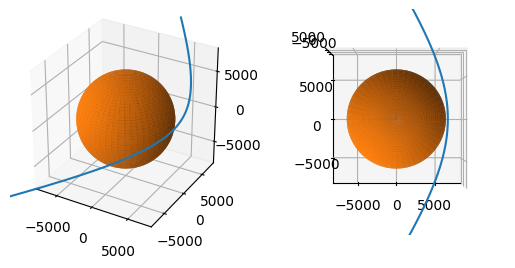
\includegraphics[width=1\linewidth]{images/coordinates_graph.png}
        \caption{Реальные параметры}
    \end{subfigure}
    \begin{subfigure}{0.5\textwidth}
        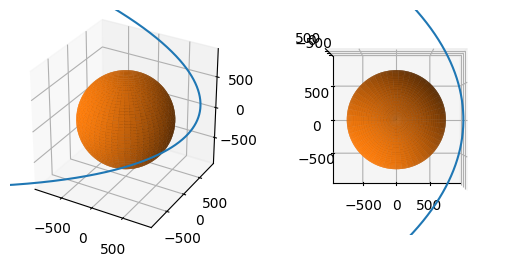
\includegraphics[width=1\linewidth]{images/eve_coordinates.png}
        \caption{Ева}
        \label{fig:enter-label}
    \end{subfigure}
    \caption{Графики координат}
    \end{figure}
    Посчитаем модуль скорости и объединим массивы с временем:
    \begin{minted}{python}
        v = np.linalg.norm(y[3:], axis=0) / 1000
        t = np.concatenate([np.flip(t_minus_eval, axis=0), t_plus_eval[1:]]) / 60
    \end{minted}
    И выведем график скорости:
    \begin{minted}{python}
        plt.plot(t, v)
        plt.title("Скорость аппарата")
        plt.ylabel("Скорость, км/с")
        plt.xlabel("Время относительно T0, мин")
        plt.show()
    \end{minted}
    \begin{figure}[H]
    \begin{subfigure}{0.5\textwidth}
        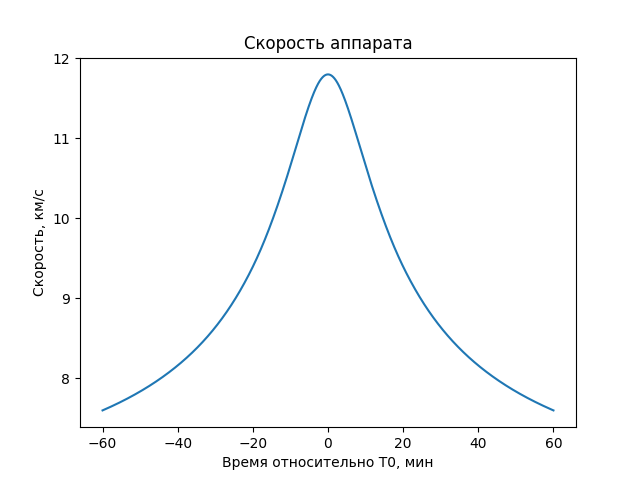
\includegraphics[width=1\linewidth]{images/speed_graph.png}
        \caption{Реальные параметры}
    \end{subfigure}
    \begin{subfigure}{0.5\textwidth}
        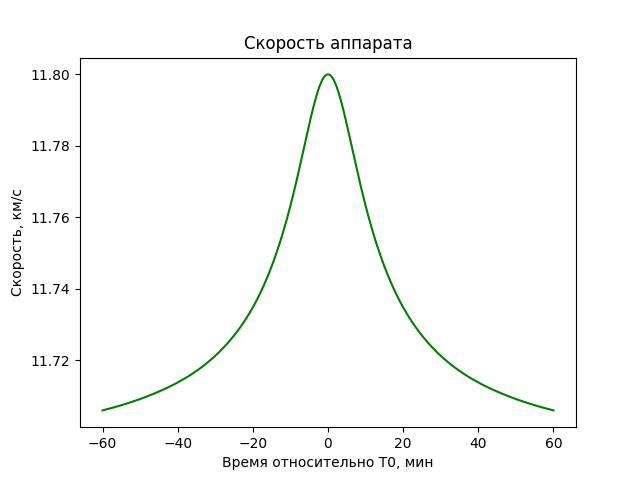
\includegraphics[width=1\linewidth]{images/eve_speed.png}
        \caption{Ева}
    \end{subfigure}
    \caption{Графики скорости}
    Также сохраним результаты на будущее:
    \begin{minted}{python}
    import joblib

    joblib.dump(v, '../data/math_v.joblib')
    joblib.dump(t, '../data/math_t.joblib')
    joblib.dump(y, '../data/math_y.joblib')
    \end{minted}
    \end{figure}
    \subsection{KSP}
    \subsubsection{Снятие данных}
    Для того, чтобы приблизить условия в KSP к реальным, мы решили задать орбиту вручную через cheat menu(alt-f12):
     \begin{figure}[H]
         \centering
         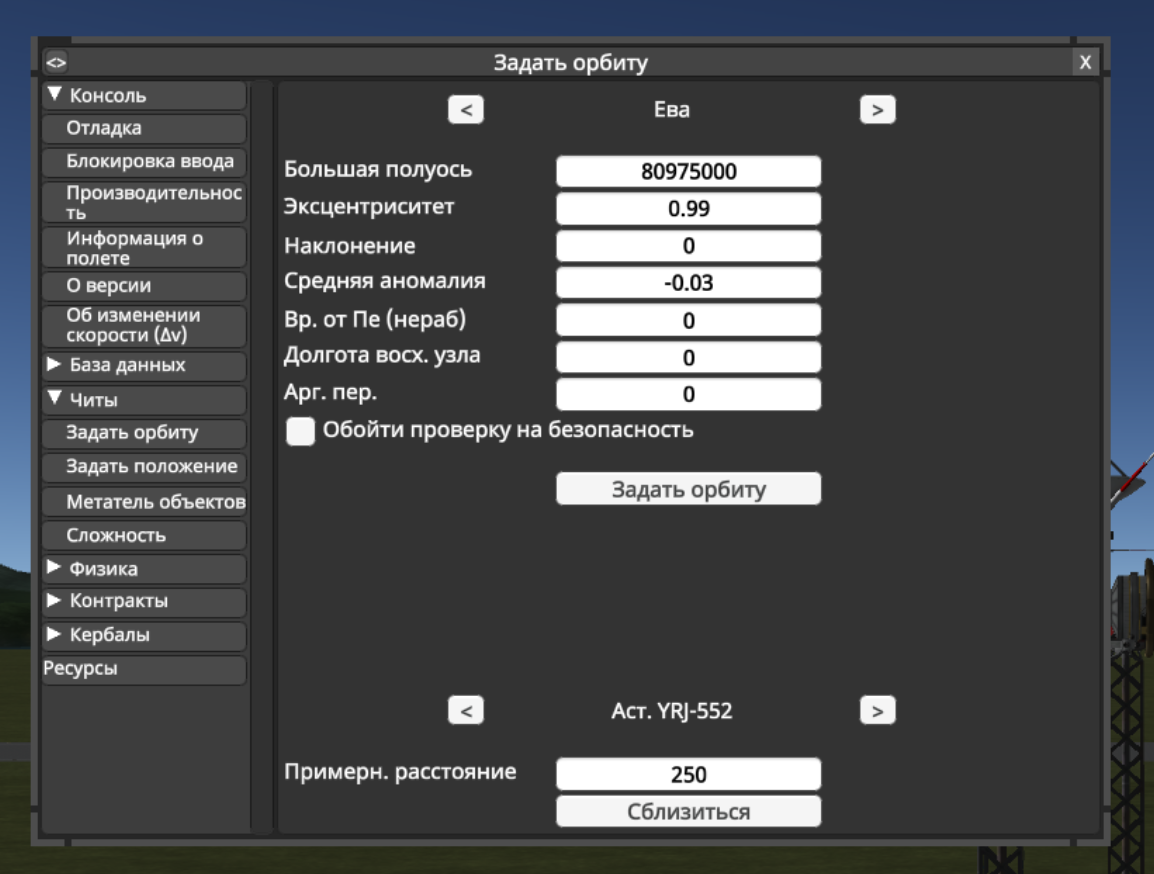
\includegraphics[width=0.5\linewidth]{images/orbit_params.png}
         \caption{Паметры орбиты}
         \label{fig:enter-label}
     \end{figure}
     После чего с помощью библиотеки krpc мы автоматически выполняем маневр для увеличения перигея орбиты до 248 км. Дальше мы включем ускорение времени 10x и начинаем снимать данные о скорости и координате до завершения программы. При остановке массивы с данными сохраняются с помощью библиотеки joblib:
     \begin{minted}{python}
    import os
    import time
    import krpc
    import matplotlib.pyplot as plt
    import joblib
    
    DATA_PATH = '../../data/'
    if not os.path.exists(DATA_PATH):
        os.mkdir(DATA_PATH)
    conn = krpc.connect()
    
    spc = conn.space_center
    vessel = conn.space_center.active_vessel
    vessel.control.activate_next_stage()
    
    vessel.control.sas = True
    time.sleep(1)
    for _ in range(100):
        vessel.control.sas_mode = vessel.control.sas_mode.prograde
    time.sleep(1)
    vessel.control.throttle = 1.0
    
    periapsis_altitude = conn.get_call(getattr, vessel.orbit, 'periapsis_altitude')
    expr = conn.krpc.Expression.greater_than(
        conn.krpc.Expression.call(periapsis_altitude),
        conn.krpc.Expression.constant_double(250000))
    event = conn.krpc.add_event(expr)
    with event.condition:
        event.wait()
    vessel.control.throttle = 0
    # Начинаем снимать данные
    velocities = []
    cords = []
    times = []
    position = conn.add_stream(vessel.position, vessel.orbit.body.reference_frame)
    velocity = conn.add_stream(getattr, vessel.flight(
        vessel.orbit.body.reference_frame), 'speed')
    ut = conn.add_stream(getattr, conn.space_center, 'ut')
    
    work = True
    try:
        time.sleep(2)
        for _ in range(1000):
            spc.rails_warp_factor = 3
        while work:
            cords.append(position())
            velocities.append(velocity())
            times.append(ut())
            time.sleep(0.1)
    except KeyboardInterrupt:
        spc.rails_warp_factor = 0
        joblib.dump(cords, os.path.join(DATA_PATH, "cords.joblib"))
        joblib.dump(velocities, os.path.join(DATA_PATH, "velocities.joblib"))
        joblib.dump(times, os.path.join(DATA_PATH, "time.joblib"))
        work = False
        plt.plot(velocities)
        plt.show()
        exit(0)

     \end{minted}
     \subsubsection{Анализ данных}
     Для того, чтобы вывести график скорости нужно полученные данные предварительно обработать. Сначала загрузим массивы с помощью joblib:
     \begin{minted}{python}
     velocities = np.array(joblib.load(os.path.join(DATA_PATH, "velocities.joblib")))
     times = np.array(joblib.load(os.path.join(DATA_PATH, "time.joblib")))
     \end{minted}
     Теперь возьмем найдем индекс, в котором скорость достигает максимума и вычтем время по этому индексу из каждого элемента массива, а потом переведем время в минуты:
     \begin{minted}{python}
     times -= times[np.argmax(velocities)]
     times /= 60
     \end{minted}
     Найдем все индексы, которые входят в заранее заданный диапазон времени:
     \begin{minted}{python}
     index_in_time_range = np.argwhere(np.abs(times) <= TIME_RANGE * 60)
     \end{minted}
     Построим график:
     \begin{minted}{python}
     plt.plot(times[index_in_time_range], velocities[index_in_time_range], 'r')
     plt.title("Скорость аппарата в KSP")
     plt.ylabel("Скорость, км/с")
     plt.xlabel("Время относительно T0, мин")
     plt.show()
     \end{minted}
     \begin{figure}[H]
         \centering
         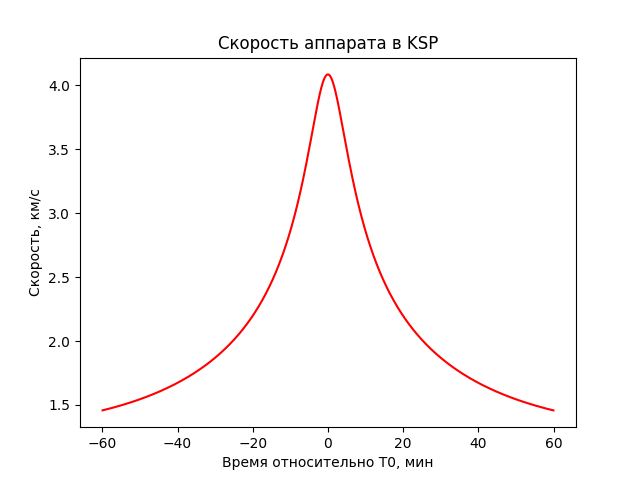
\includegraphics[width=0.5\linewidth]{images/ksp_speed.png}
         \caption{Скорость в KSP}
     \end{figure}
    \section{Сравнение результатов и выводы}
    Для сравнения модели и KSP загрузим сохраненные результаты:
    \begin{minted}{python}
    math_v = joblib.load(os.path.join(DATA_PATH, "math_v.joblib"))
    math_t = joblib.load(os.path.join(DATA_PATH, "math_t.joblib"))
    \end{minted}
    Выведем сравнительный график:
    \begin{minted}{python}
        plt.plot(times[index_in_time_range], velocities[index_in_time_range], 'r', label='KSP')
    plt.plot(math_t, math_v, 'g', label='Модель')
    plt.title("Сравнение модели и KSP")
    plt.ylabel("Скорость, км/с")
    plt.xlabel("Время относительно T0, мин")
    plt.legend(loc='best')
    plt.show()
    \end{minted}
    \begin{figure}
        \centering
        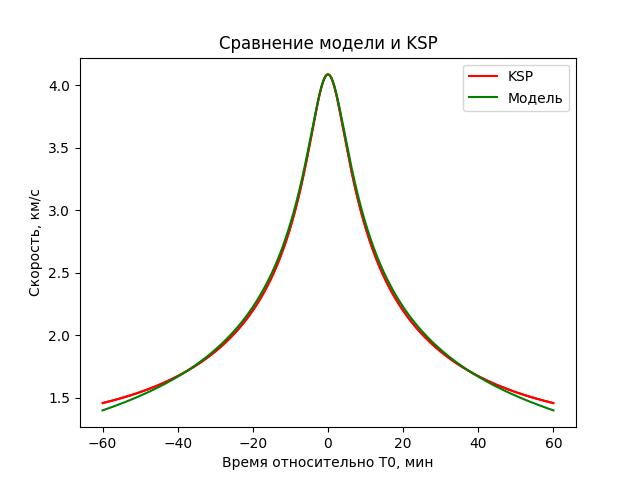
\includegraphics[width=0.75\linewidth]{images/compare_math_ksp_speed.png}
        \caption{Сравнительный график}
        \label{fig:compare}
    \end{figure}
    По рис. \ref{fig:compare} видно, что модель очень близко повторяет график скорости в KSP, из чего можно сделать вывод, что мы смогли построить достаточно точную модель.
    \newpage
    \nocite{*}
    \printbibliography
\end{document}